\documentclass[a4paper, 12pt]{article}

\usepackage[top=2cm, bottom=3cm, right=2cm, left=2cm]{geometry}
\usepackage[utf8]{inputenc}
\usepackage{amsmath, amsfonts, amssymb}
\usepackage{float}
\usepackage{graphicx}
\usepackage[portuguese]{babel}
\usepackage{listings}

\title{Cálculo Numérico

Atividade avaliativa 2
}
\author{Luís Otávio Lopes Amorim}


\begin{document}
\maketitle

\begin{enumerate}

	\item Em um determinado experimento foram observados os seguintes dados:
	\begin{center}
	\begin{tabular}{|c|c|c|c|c|}
		\hline
		$x_i$ & $-2$ & $0$ & $1$ & $3$ \\ \hline
		$y_i$ & $-1$ & $1$ & $-2$ & $-1$ \\ \hline
	\end{tabular}
	\end{center}
	
	Sabendo que o comportamenteo da função que descreve
	tal fenômeno é semelhante ao de uma função polinomial
	de grau 3, pede-se:
	
	\begin{enumerate}
		\item \textbf{(4,0)} Faça, pelo método dos mínimos quadrados,
		o ajuste da curva que descreve o fenômeno observado por uma
		função da forma $f(x) = ax^3+bx^2+cx+d$.
		
		\begin{center} \textbf{SOLUÇÃO} \\ \end{center}
		O exercício pede a função $$\varphi (x) = \alpha x^3 + \beta x^2  \gamma x + \theta$$.
		Assim, temos as funções $g(x)$:
		$$g_1(x) = x^0$$
		$$g_2(x) = x^1$$
		$$g_3(x) = x^2$$
		$$g_4(x) = x^3$$
		
		Portanto, para encontrar os coeficientes $\alpha$ $\beta$ $\gamma$ e $\theta$
		basta resolver o sistema:
		\\ \\
		$$	
		\left\{
		\begin{array}{cccc}
		
		\displaystyle	
		\alpha \sum_{k=1}^4x_k^0 + 	\beta \sum_{k=1}^4x_k^1 +
		\gamma \sum_{k=1}^4x_k^2 + \theta \sum_{k=1}^4x_k^3 = \sum_{k=1}^4 x_k^0 \cdot y_k	\\
		
		\displaystyle
		\alpha \sum_{k=1}^4x_k^1 + 	\beta \sum_{k=1}^4x_k^2 +
		\gamma \sum_{k=1}^4x_k^3 + \theta \sum_{k=1}^4x_k^4 = \sum_{k=1}^4x_k^1 \cdot y_k \\
		
		\displaystyle
		\alpha \sum_{k=1}^4x_k^2 + 	\beta \sum_{k=1}^4x_k^3 +
		\gamma \sum_{k=1}^4x_k^4 + \theta \sum_{k=1}^4x_k^5 = \sum_{k=1}^4 x_k^2 \cdot y_k \\
		
		\displaystyle
		\alpha \sum_{k=1}^4x_k^3 + 	\beta \sum_{k=1}^4x_k^4 +
		\gamma \sum_{k=1}^4x_k^5 + \theta \sum_{k=1}^4x_k^6 = \sum_{k=1}^4 x_k^3 \cdot y_k
		
		\end{array}
		\right. $$
		
		Assim, primeiro devemos calcular os somatórios:
		
		\begin{center}
		\begin{tabular}{ccccc}
			$\displaystyle \sum_{k=1}^4x_k^0 = 4$ & $\displaystyle \sum_{k=1}^4x_k^1 = 2$ &
			$\displaystyle \sum_{k=1}^4x_k^2 = 14$ & $\displaystyle \sum_{k=1}^4x_k^3 = 20$
			& $\displaystyle \sum_{k=1}^4x_k^4 = 98$ \\
			
			$\displaystyle \sum_{k=1}^4x_k^5 = 212$ & $\displaystyle \sum_{k=1}^4x_k^6 = 794$ &
			$\displaystyle \sum_{k=1}^4x_k^0 \cdot y_k = -3$ &
			$\displaystyle \sum_{k=1}^4x_k^1 \cdot y_l = -3$ &
			$\displaystyle \sum_{k=1}^4x_k^2 \cdot y_k = -15$ \\
			$\displaystyle \sum_{k=1}^4x_k^3 \cdot y_k = -21$  
		\end{tabular}
		\end{center}
		
		Para então criar a matriz dos coeficientes e escaloná-la:
		
		$$
		\begin{pmatrix}
			4 & 2 & 14 & 20 & -3 \\
			2 & 14 & 20 & 98 & -3 \\
			14 & 20 & 98 & 212 & -15 \\
			20 & 98 & 212 & 794 & -21
		\end{pmatrix}
		\begin{matrix}
			\\ L_2 = 2L_2 - L_1 \\ L_3 = 2L_3 - 7 L_1 \\ L_4 = L_4 - 5L_1
		\end{matrix} \sim
		\begin{pmatrix}
			4 & 2 & 14 & 20 & -3 \\
			0 & 26 & 26 & 176 & -3 \\
			0 & 26 & 98 & 284 & -9 \\
			0 & 88 & 142 & 694 & -6
		\end{pmatrix}				
		$$
		
		$$
		\begin{pmatrix}
			4 & 2 & 14 & 20 & -3 \\
			0 & 26 & 26 & 176 & -3 \\
			0 & 26 & 98 & 284 & -9 \\
			0 & 44 & 71 & 347 & -3
		\end{pmatrix}
		\begin{matrix}
			\\  \\ L_3 = L_3 - L_3 \\ L_4 = 13L_4 - 22L_2
		\end{matrix} \sim		
		\begin{pmatrix}
			4 & 2 & 14 & 20 & -3 \\
			0 & 26 & 26 & 176 & -3 \\
			0 & 0 & 72 & 108 & -6 \\
			0 & 0 & 351 & 639 & 27
		\end{pmatrix}				
		$$
		
		$$
		\begin{pmatrix}
			4 & 2 & 14 & 20 & -3 \\
			0 & 26 & 26 & 176 & -3 \\
			0 & 0 & 12 & 18 & -1 \\
			0 & 0 & 39 & 71 & 3
		\end{pmatrix}
		\begin{matrix}
			\\  \\  \\ L_4 = 4L_4 - 13L_2
		\end{matrix} \sim		
		\begin{pmatrix}
			4 & 2 & 14 & 20 & -3 \\
			0 & 26 & 26 & 176 & -3 \\
			0 & 0 & 12 & 18 & -1 \\
			0 & 0 & 0 & 50 & 25
		\end{pmatrix}			
		$$
		
		Assim, temos: 
		
		$$\alpha = \frac{1}{2} \, \beta = \frac{-5}{6} \, \gamma = \frac{-8}{3} \, \theta = 1$$
		
		Então:
		$$\varphi (x) = \frac{x^3}{2} - \frac{5x^2}{6} - \frac{8x}{3} + 1$$
		\\ \\
		\item \textbf{(3,0)} Construa o gráfico da função encontrada e calcule o erro quadrático envolvido no processo.
		
		\begin{center} \textbf{SOLUÇÃO} \\ \end{center}
		
		Observando o gráfico, podemos perceber que todos os
		pontos tabelados estão presentes no gráfico.
		Assim, $f(x_k) - \varphi (x_k) = 0$ para todo k. Portanto, o erro quadrático é 0.
		
		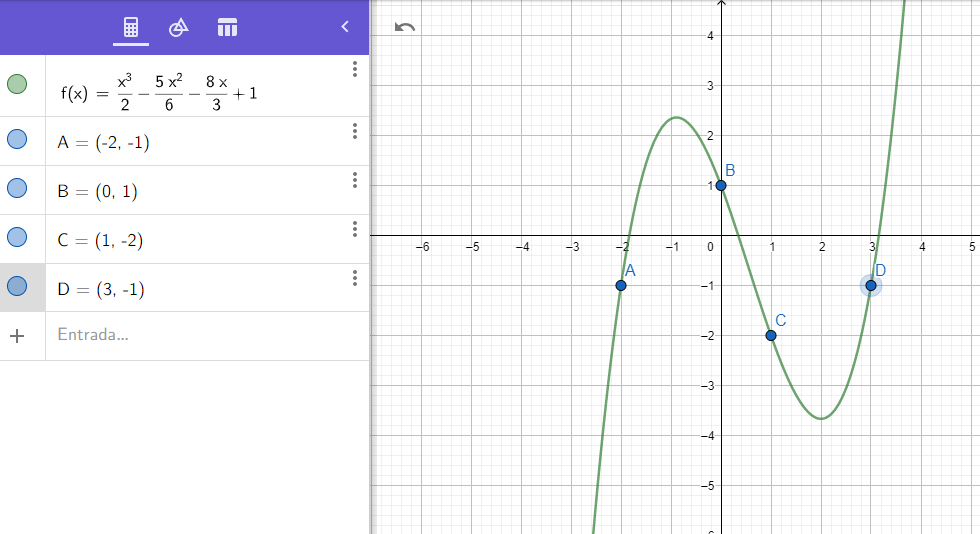
\includegraphics[scale=.5]{grafico}		
		\\ \\
		\item \textbf{(3,0)} Usando um software e um método de sua escolha (dentre os três métodos
		vistos em aula), contrua um algoritmo e calcule TODAS as raízes de f(x) com precisão de 0,001.
		
		\begin{center} \textbf{SOLUÇÃO} \\ \end{center}

		\lstinputlisting[language=C]{ex.c}
	\end{enumerate}
\end{enumerate}
\end{document}